\documentclass{standalone}
\usepackage[dvipsnames]{xcolor}
\usepackage{tikz}
\usetikzlibrary{positioning,calc,fit
  ,matrix
  ,chains,scopes}


\definecolor{mybluei}{RGB}{124,156,205}
\definecolor{myblueii}{RGB}{73,121,193}
\definecolor{mygreen}{RGB}{202,217,126}
\definecolor{mypink}{RGB}{233,198,235}


\pgfdeclarelayer{background}
\pgfsetlayers{background,main}

\pgfkeys{
  /tikz/node distance/.append code={
    \pgfkeyssetvalue{/tikz/node distance value}{#1}
  }
}




\tikzset{
  tikzcomputerpic/.style={ 
    node distance=20pt
    ,inner sep=0pt
    ,outer sep=0pt
  }
  ,title/.style={ inner sep=0pt, color=white}
  ,bounder/.style={rounded corners,draw=black,inner sep=5pt}
  ,computer/.style={bounder,fill=gray!20}
  ,computername/.style={
    ,font=\ttfamily\color{black}
     ,above=25pt of stack
    ,remember picture
  }
  ,blueb/.style={
    draw=white, line width=.5pt,
    fill=myblueii,
    text width=2.6cm,
    font={\sffamily\color{white}},
    align=center,
    text height=12pt,
    text depth=9pt
  }
  ,span/.style={inner sep=0pt,text height=12pt}
  ,dockerapp/.style={blueb,fill=mybluei,font={\sffamily\bfseries\color{white}}}
  ,docker/.style={blueb,fill=myblueii}
  ,os/.style={blueb,fill=BurntOrange,font={\sffamily\color{black}}}
  ,stack/.style={ column sep=0em, row sep=0em}
  ,sharestyle/.style={blueb,fill=Aquamarine}
  ,app/.style={blueb,fill=Periwinkle}
  ,vagrantcomputer/.style={computer,fill=Periwinkle!15}
  ,zone/.style={rectangle
    ,dashed
    ,very thick
    ,draw=black
    ,inner sep=.2in}
}


\newcommand\shareblock[2][\texttt{/project}]{
\node[sharestyle] (#2) {#1};
}


\begin{document}
\begin{tikzpicture}[
node distance=.2in
,inner sep=0in
,remember picture
]



\node[] (local) {
  \begin{tikzpicture}[tikzcomputerpic]
    % local computer
    \matrix[stack](stack){
      \node[dockerapp] (localapp3) {app3}; 
      & \node[app](localvirtualbox) {VirtualBox};
      \\
      \node[docker] (localdkr) {Docker};
      & \node[app](localvagrant) {Vagrant};
      & \shareblock[share:\texttt{/project}]{localshare}
      \\
      \node[os] (localos1) {}; 
      & \node[os] (localos2) {}; 
      & \node[os] (localos3) {};
      \\
    };
    \node[os,fit=(localos1)(localos2)(localos3),span]
    (localos)
    {Win\textbar Lin\textbar OSX}; 
    \node[computername] (localnm) {localhost};
    \begin{pgfonlayer}{background}
      \node[computer,fit=(localnm) (stack)] (localbox) {};
    \end{pgfonlayer}
  \end{tikzpicture}
};



\node[above= of local,yshift=1in ] (init) {
  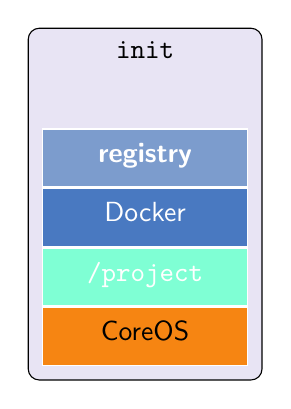
\begin{tikzpicture}[tikzcomputerpic]
    % init computer
    \matrix[stack](stack){
      \node[dockerapp] (initreg) {registry};
      \\
      \node[docker] (initdkr) {Docker}; 
      \\
      \shareblock{initshare};
      \\
      \node[os] (initos) {CoreOS}; 
      \\
    };
    \node[computername] (initnm) {init};
    \begin{pgfonlayer}{background}
      \node[vagrantcomputer
      ,fit=(initnm) (stack)
      ] (initbox) {};
    \end{pgfonlayer}
  \end{tikzpicture}
};


%alignment of compute nodes along bottom
{[start chain=computemachines going base right]


\node[above = of init,on chain] (vagrant) {
  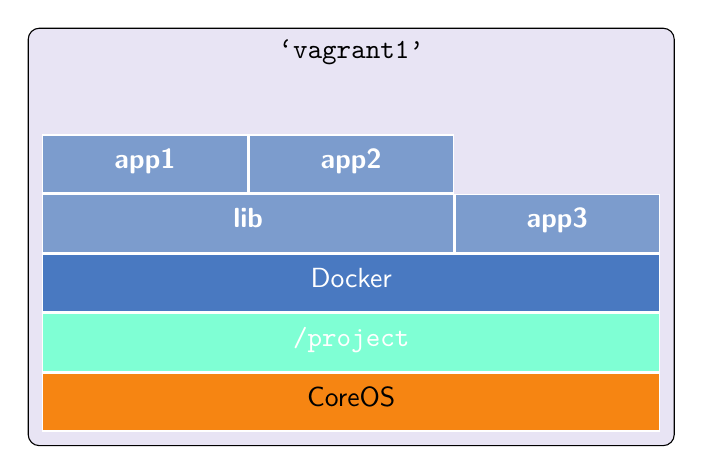
\begin{tikzpicture}[tikzcomputerpic]
    % vagrant compute computer
    \matrix[stack](stack){
      \node[dockerapp] (vagapp1) {app1}; 
      & \node[dockerapp] (vagapp2) {app2}; 
      \\
      \node[dockerapp] (vaglib1) {};
      & \node[dockerapp] (vaglib2) {};
      & \node[dockerapp] (vagapp3) {app3}; 
      \\
      \node[docker] (vagdkr1) {};
      & \node[docker] (vagdkr2) {};
      & \node[docker] (vagdkr3) {};
      \\
      \node[sharestyle] (vagshare1) {};
      & \node[sharestyle] (vagshare2) {};
      & \node[sharestyle] (vagshare3) {};
      \\
      \node[os] (vagos1) {};
      & \node[os] (vagos2) {};
      & \node[os] (vagos3) {};
      \\
    };


    % span is last
    \node[dockerapp,fit= (vaglib1) (vaglib2),span] (vag1lib) {lib};
    \node[sharestyle,fit= (vagshare1) (vagshare2)(vagshare3),span]
    (vagshare) {\texttt{/project}};
    \node[docker,fit=(vagdkr1)(vagdkr2)(vagdkr3),span ] (vagdkr) {Docker}; \\
    \node[os,fit=(vagos1)(vagos2)(vagos3),span ] (vagos) {CoreOS}; \\
    \node[computername] (vagrantcomputenm) {`vagrant1'};

    \begin{pgfonlayer}{background}
      \node[vagrantcomputer
      ,fit=(vagrantcomputenm) (stack)] (vagrantcomputebox) {};
    \end{pgfonlayer}
  \end{tikzpicture}
};




\node[on chain] (vagrant2) {
  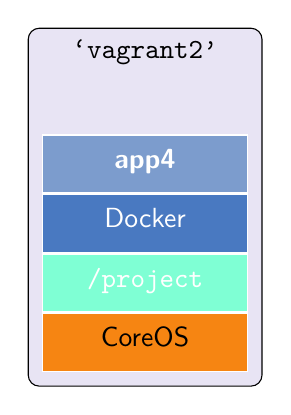
\begin{tikzpicture}[tikzcomputerpic]
    % init computer
    \matrix[stack](stack){
      \node[dockerapp] (vag2app4) {app4};
      \\
      \node[docker] (vag2dkr) {Docker}; 
      \\
      \shareblock{vag2share};
      \\
      \node[os] (vag2os) {CoreOS}; 
      \\
    };
    \node[computername] (vag2nm) {`vagrant2'};
    \begin{pgfonlayer}{background}
      \node[vagrantcomputer
      ,fit=(vag2nm) (stack)] (vag2box) {};
    \end{pgfonlayer}
  \end{tikzpicture}
};



\node[on chain,xshift=1.5in] (aws1) {
  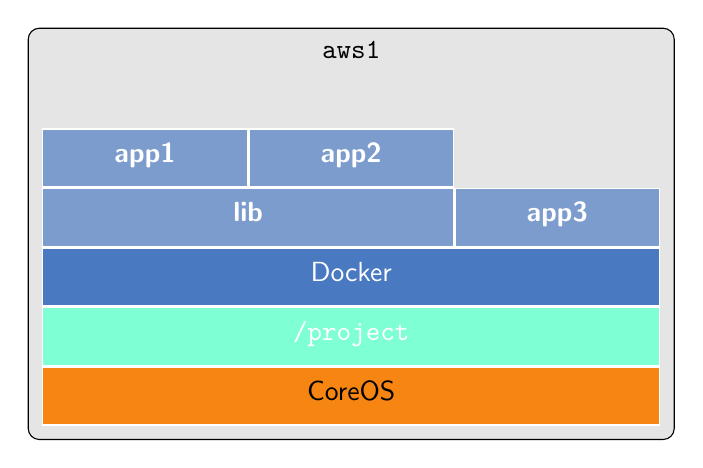
\begin{tikzpicture}[tikzcomputerpic]
    % vagrant compute computer
    \matrix[stack](stack){
      \node[dockerapp] (aws1app1) {app1}; 
      & \node[dockerapp] (aws1app2) {app2}; 
      \\
      \node[dockerapp] (aws1lib1) {};
      & \node[dockerapp] (aws1lib2) {};
      & \node[dockerapp] (aws1app3) {app3}; 
      \\
      \node[docker] (aws1dkr1) {};
      & \node[docker] (aws1dkr2) {};
      & \node[docker] (aws1dkr3) {};
      \\
      \node[sharestyle] (aws1share1) {};
      & \node[sharestyle] (aws1share2) {};
      & \node[sharestyle] (aws1share3) {};
      \\
      \node[os] (aws1os1) {};
      & \node[os] (aws1os2) {};
      & \node[os] (aws1os3) {};
      \\
    };


    % span is last
    \node[dockerapp,fit= (aws1lib1) (aws1lib2),span] (aws1lib) {lib};
    \node[sharestyle,fit= (aws1share1) (aws1share2)(aws1share3),span]
    (aws1lib) {\texttt{/project}};
    \node[docker,fit=(aws1dkr1)(aws1dkr2)(aws1dkr3),span ] (aws1dkr) {Docker}; \\
    \node[os,fit=(aws1os1)(aws1os2)(aws1os3),span ] (aws1os) {CoreOS}; \\
    \node[computername] (aws1nm) {aws1};

    \begin{pgfonlayer}{background}
      \node[computer
      ,fit=(aws1nm) (stack)] (aws1box) {};
    \end{pgfonlayer}
  \end{tikzpicture}
};



\node[on chain] (aws2) {
  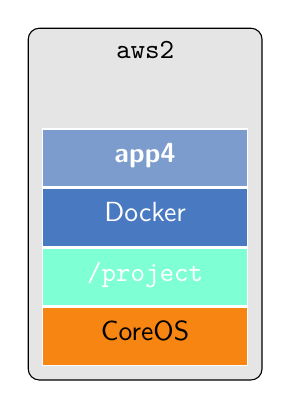
\begin{tikzpicture}[tikzcomputerpic]
    % init computer
    \matrix[stack](stack){
      \node[dockerapp] (aws2app4) {app4};
      \\
      \node[docker] (aws2dkr) {Docker}; 
      \\
      \shareblock{aws2share};
      \\
      \node[os] (aws2os) {CoreOS}; 
      \\
    };
    \node[computername] (aws2nm) {aws2};
    \begin{pgfonlayer}{background}
      \node[computer,fit=(aws2nm) (stack)] (aws2box) {};
    \end{pgfonlayer}
  \end{tikzpicture}
};

}



%zones

\node[zone,inner sep=0pt
,fit= (vagapp1)  (aws2app4)
,color=mybluei
,dotted
,label=below:\textsf{Weave Net}
] (weavenet) {};

\node[zone
,fit= (vagrant) (init) (vagrant2)
,label=below:\textsf{VirtualBox}/\textsf{Vagrant}
,color=Periwinkle
] (vagrantgrp) {};

\node[zone
,fit=(init) (local) (vagrantgrp)
,label=below:local
] {};

\node[zone
,fit= (aws1) (aws2)
,label=below:remote (AWS)
] {};



%weave connections
%http://hugoideler.com/2013/01/tikz-node-connector/
% \newcommand*{\connectorH}[4][]{
%   \draw[#1] (#3)
%   node[right=20pt of initshare,above] {\textsf{Weave}}
%   -| ($(#3) !#2! (#4)$)
%   |- (#4)
% ;
% }
% \newcommand*{\connectorV}[4][]{
%   \draw[#1] (#3) |- ($(#3) !#2! (#4)$) -| (#4);
% }
% \connectorH[thick]{.5}{localshare}{initshare}

\end{tikzpicture}
\end{document}
